% $Header: /cvsroot/latex-beamer/latex-beamer/examples/beamerexample1.tex,v 1.47 2004/11/04 15:43:51 tantau Exp $

\documentclass{beamer}
%\documentclass{article}
%\usepackage[envcountsect]{beamerarticle}

% Do NOT take this file as a template for your own talks. Use a file
% in the directory solutions instead. They are much better suited.

% Try the class options [notes], [notes=only], [trans], [handout],
% [red], [compress], [draft] and see what happens!

% Copyright 2003 by Till Tantau <tantau@users.sourceforge.net>.
%
% This program can be redistributed and/or modified under the terms
% of the LaTeX Project Public License Distributed from CTAN
% archives in directory macros/latex/base/lppl.txt.

% For a green structure color use:
%\colorlet{structure}{green!50!black}

\usepackage{array,paralist}
\usepackage{tabularx}
\usepackage{eurosym}

\mode<article> % only for the article version
{
  \usepackage{fullpage}
  \usepackage{hyperref}
}


\mode<presentation>
{
  \setbeamertemplate{background canvas}[vertical shading][bottom=red!10,top=blue!10]

  \usetheme{CambridgeUS}
  \usefonttheme[onlysmall]{structurebold}
}

%\setbeamercolor{math text}{fg=green!50!black}
%\setbeamercolor{normal text in math text}{parent=math text}

\usepackage{amsmath,amssymb}
\usepackage[latin1]{inputenc}
\usepackage{colortbl}
\usepackage[english]{babel}

%\usepackage{lmodern}
%\usepackage[T1]{fontenc} 

\usepackage{times}
\setbeamercovered{dynamic}

%% Titel etc
\title[Patienten unter Strom: Mein erstes EKG]{Eine kurze Einf�hrung in die biomedizinische Me�technik}
\author[Noe]{Marcel Noe}
\institute[TNG]{
        \inst{}TNG Technology Consulting GmbH}
\date[2012]


%% Hauptseite
\begin{document}
\frame{\titlepage}

\section<presentation>*{Einf�hrung}

\begin{frame}
  \frametitle{�berblick}
  \tableofcontents[part=1,hidesubsections]
\end{frame}

\part<presentation>{Vortrag}


\logo{}
\section{Einf�hrung}
\subsection{Motivation}
\begin{frame}
    \frametitle{Intensivstation}

    \begin{columns}[T]
        \begin{column}{5cm}
            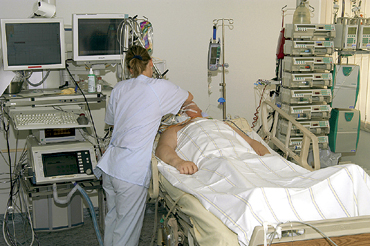
\includegraphics[width=5cm]{images/its.jpg}
        \end{column}

        \begin{column}{7cm}
            \begin{itemize}
                \item Foo 
                \item Bar 
                \item Foobar 
            \end{itemize}
        \end{column}
    \end{columns}
\end{frame}

\subsection{Triage}
\begin{frame}
    \frametitle{Motivation: Triage}

    \begin{columns}[T]
         \begin{column}{8cm}
            \begin{itemize}
                \item Bar
                \item Foo
                \item Bar
            \end{itemize}
        \end{column}

       \begin{column}{3cm}
        \end{column}
    \end{columns}

    \vspace{0.3cm} \begin{center}{\bf $\Longrightarrow$ Technische Hilfsmittel k�nnen Fehler verringern.}\end{center}
\end{frame}

\section{Medizinische Grundlagen}
\subsection{Anatomie des Menschen: Nerven}
\begin{frame}
    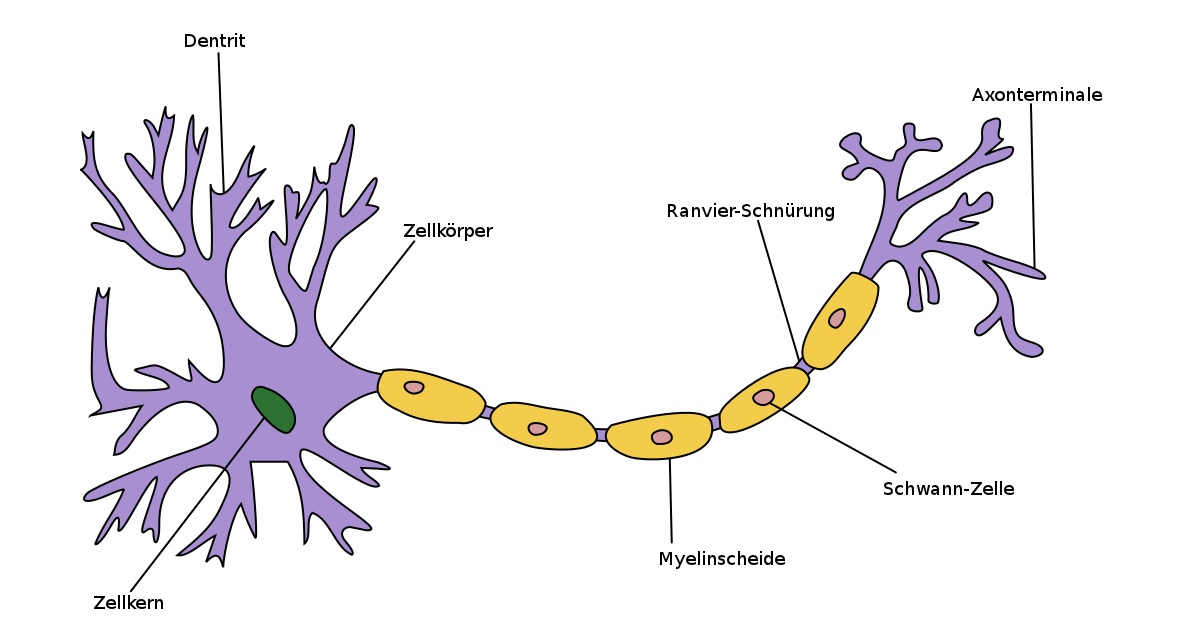
\includegraphics[width=12cm]{images/Neuron_Hand-tuned-text.jpg}
\end{frame}

\begin{frame}
    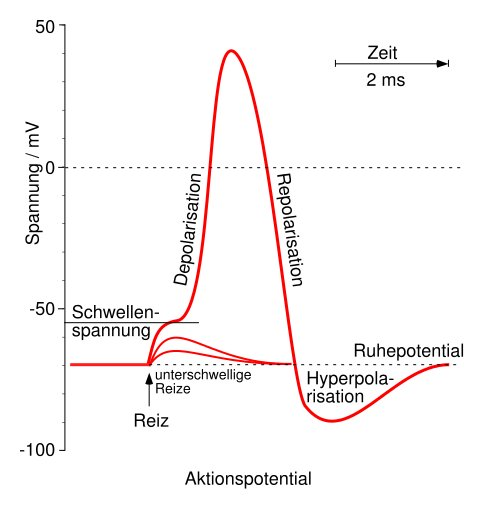
\includegraphics[height=8cm]{images/Aktionspotential.jpg}
\end{frame}

\begin{frame}
    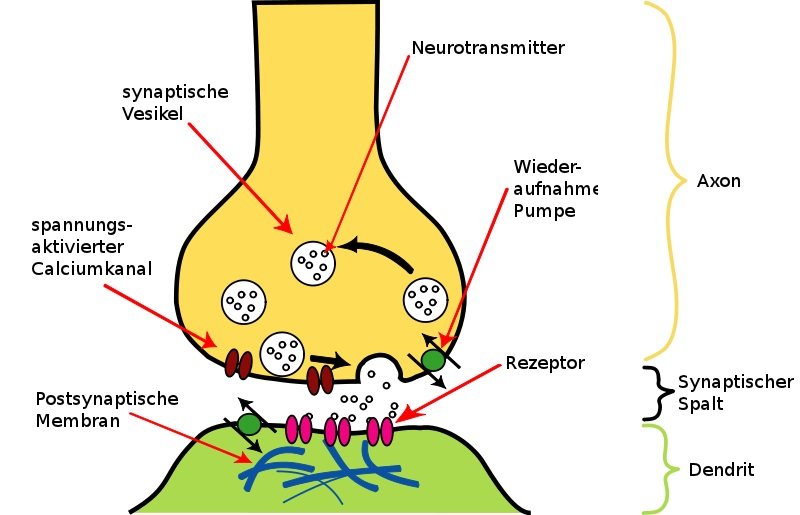
\includegraphics[height=7.5cm]{images/synaptischer_spalt.jpg}
\end{frame}


\subsection{Anatomie des Menschen: Blutgef��e}
\begin{frame}
    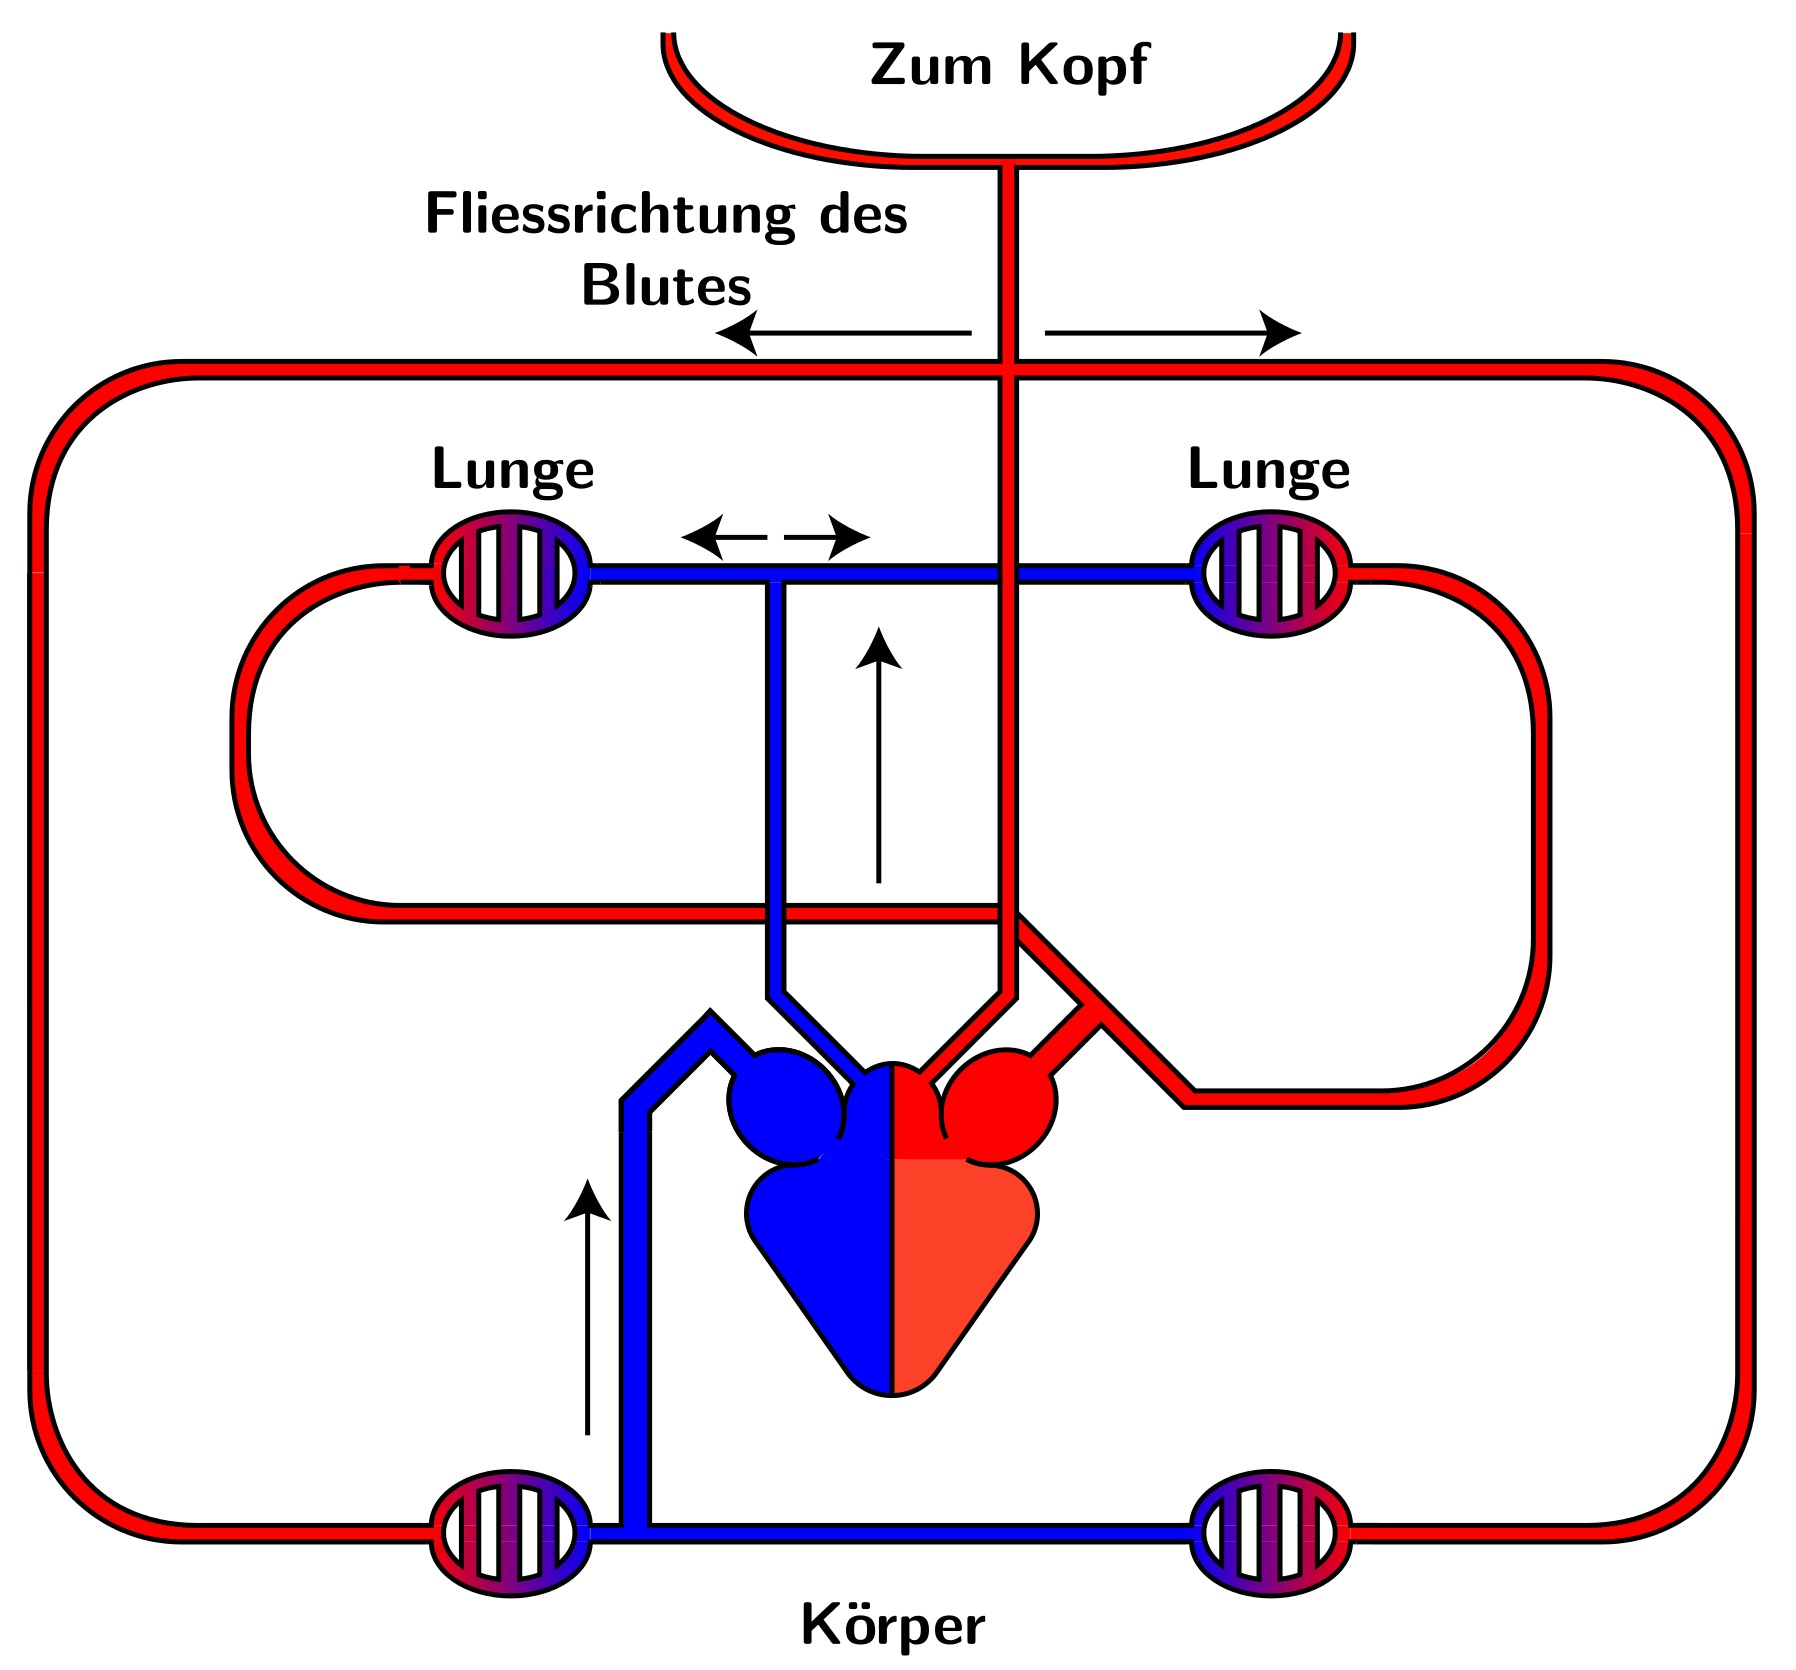
\includegraphics[height=7.5cm]{images/blutkreislauf.jpg}
\end{frame}

\subsection{Anatomie des Menschen: Herz}
\begin{frame}
    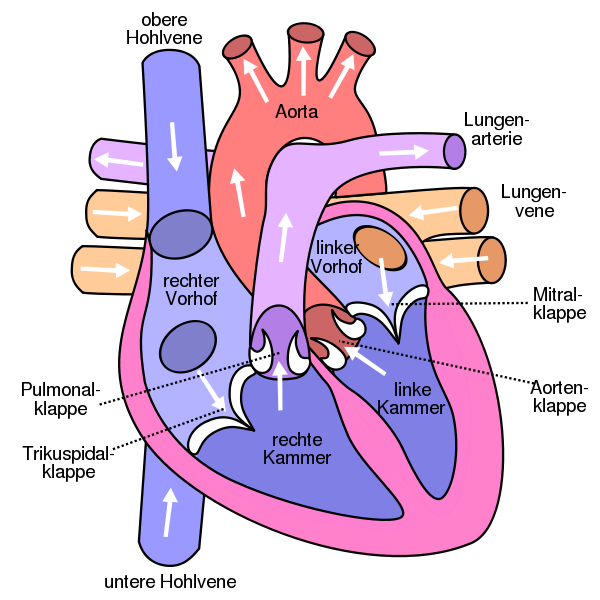
\includegraphics[height=7.5cm]{images/herz.png}
\end{frame}

\section{Messtechnik}
\subsection{Ableitung von elektrischen Signalen}
\begin{frame}
    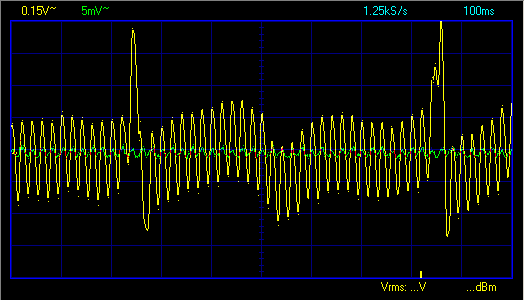
\includegraphics[height=7cm]{images/ekg_multimeter1.png}
\end{frame}

\begin{frame}
    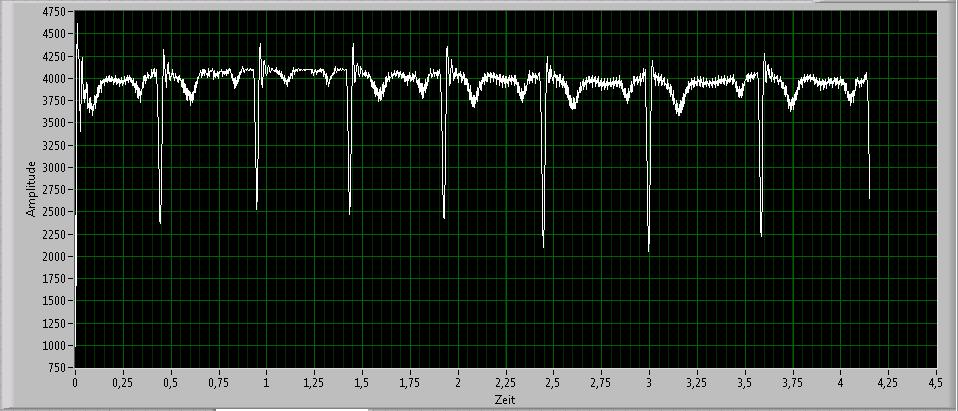
\includegraphics[width=12cm]{images/filter_notch.jpg}
\end{frame}

\begin{frame}
    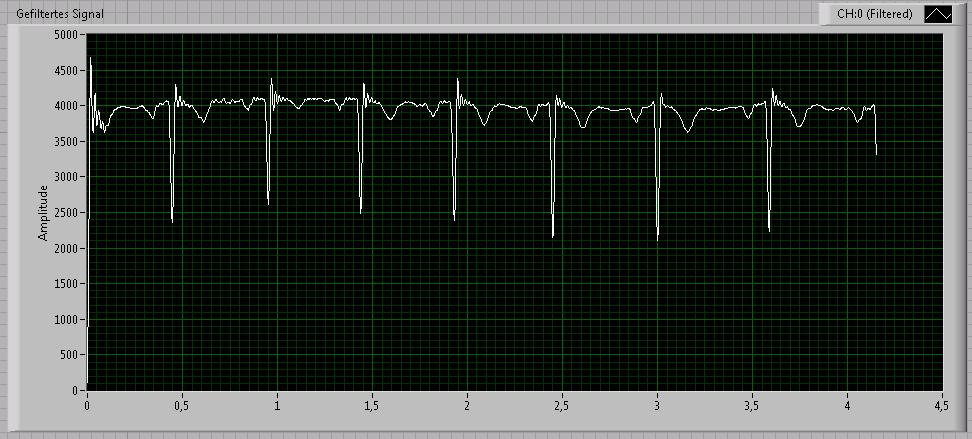
\includegraphics[width=12cm]{images/abtastrate_300.jpg}
\end{frame}

\subsection{Das EKG}
\begin{frame}
\end{frame}

\subsection{Pulsoximetrie}
\begin{frame}
\end{frame}

\subsection{Blutdruck}
\begin{frame}
\end{frame}

\subsection{Blutfluss}
\begin{frame}
\end{frame}

\subsection{Herzschritmacher}
\begin{frame}
\end{frame}

\subsection{Defibrillator}
\begin{frame}
\end{frame}

\subsection{Fragen}
\begin{frame}
    \frametitle{Fragen?}

    \begin{center}
        
\includegraphics[height=6cm]{fragezeichen.jpg}
    \end{center}
\end{frame}


\end{document}
